\begin{subsection}{Operaciones de la Arquitectura}
    El entorno ya está configurado para funcionar como un SDDC, a partir de este punto ya no es necesario realizar ninguna modificación en la infraestructura física ya que todas las tareas que se deben realizar están dentro del alcance de los componentes de VMware Cloud Foundation. Para finalizar la construcción del SDDC y habilitar un servicio donde los usuarios puedan aprovisionar recursos bajo demanda, se instalarán sobre el entorno desplegado las aplicaciones VMware vRealize Identity Manager\footnote{También se denomina Workspace ONE Access} y VMware vRealize Automation. La primera permite al administrador conectar con el servidor de usuarios y gestionarlos de forma centralizada para entregarlos a múltiples aplicaciones, como vRealize Automation, desde un mismo punto.
    
    \begin{subsubsection}{vRealize Suite Lifecycle Manager}
        
    \end{subsubsection}
    \subsubsection{Gestión del Ciclo de Vida}
    Elementos que se encargan de administrar el ciclo de vida de los componentes:
    \begin{itemize}
    %     \item \textbf{vSphere Update Manager}: por cada instancia de VMware vCenter Server se despliega una instancia de vSphere Update Manager. Este componente utiliza el servicio \textit{Update Manager Download Service} (UMDS) para obtener las actualizaciones de la red externa al SDDC, el cual se despliega en una red AVN [Fig. \ref{fig:avnConsolidated}], permitiendo limitar el acceso a Internet de vSphere Update Manager y reduciendo el número de descargas ya que un UMDS se comparte entre varias instancias de VMware vCenter Server. Se crea una instancia de UMDS por cada \textit{region} existente [Fig. \ref{fig:UpdateManagerArc}].
    %     \begin{figure}[h!]
    %         \centering
    %         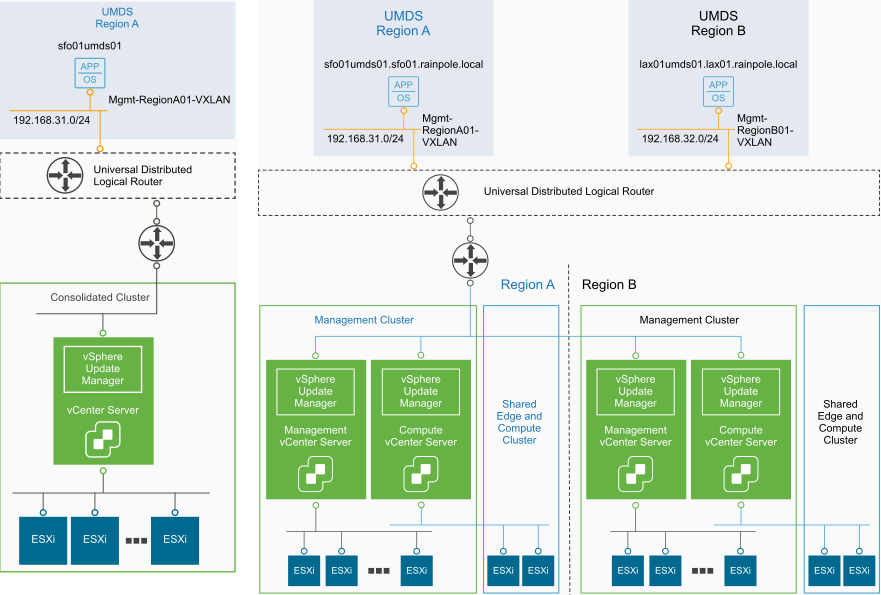
\includegraphics[width=0.5\textwidth]{imaxes/conceptosPrevios/UpdateManagerArch.png}
    %         \caption{Diseño de vSphere Update Manager en el modelo consolidado (izquierda) y en el modelo estándar (derecha)}
    %         \label{fig:UpdateManagerArc}
    %     \end{figure}
    %     \FloatBarrier
        
        \item \textbf{vRealize Suite Licfecycle Manager}: componente utilizado para desplegar, actualizar y configurar, de forma automatizada, los productos vRealize Operations, vRealize Log Insight, vRealize Automation y vRealize Business Cloud. De este componente se despliega una única instancia en una AVN accesible desde cada \textit{region} por todas las instancias de VMware vCenter Server. Se debe registrar su nombre de dominio en el servidor DNS para hacerla accesible.
        
    %     \iffalse
    %     y se puede elegir entre dos modelos de despliegue, uno en el que se usa una máquina virtual denominada  que se encarga de descargar los archivos requeridos por vSphere Update Manager mientras este se encuentra en un entorno aislado [Fig. \ref{fig:updateManager}], y otro donde es la instancia de vSphere Update Manager la que realiza la descarga de los ficheros. La primera opción incrementa la seguridad y permite compartir estos archivos entre distintas instancias de vSphere Update Manager.\\
    %     Una vez desplegado se pueden establecer diferentes configuraciones a nivel de host, máquina virtual y cluster, para que durante la instalación de actualizaciones el servicio del SDDC continúe operativo y evitar la pérdida de información y errores en los recursos.
    %     \begin{figure}[h!]
    %   \centering
    %   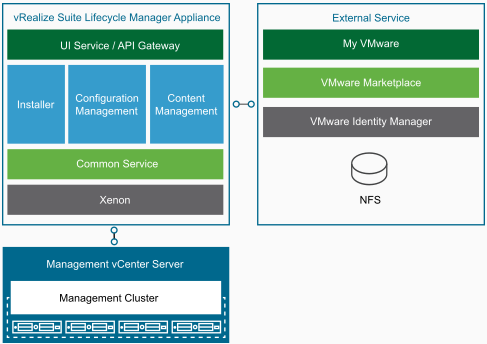
\includegraphics[width=0.8\textwidth]{imaxes/conceptosPrevios/vRealizeUpdateArchLifeCyle.png}
    %   \caption{Estructura de la gestión del ciclo de vida con vRealize Suite Lifecycle Manager.}
    %   \label{fig:vrealizeUpdateManager}
    % \end{figure}
    % \FloatBarrier
    %     \fi
    
    
    \end{itemize}
    
\end{subsection}